\section{Enumeration of vulnerable resources}

\begin{table}
  \caption{Summary of vulnerable resources \label{tab:vulnerable}}
 \centering
\begin{tabular}{l*{3}{c}}
\Xhline{2\arrayrulewidth}
\#  & \textbf{\textit{Global 1}} & \textbf{\textit{Global 2}} \\
\hline
Domains & 309,687(0.095\%) & 381,965(0.108\%) \\
NS (IP addresses) & 5738(0.166\%) & 5576(0.145\%) \\
Domain--NS IP pairs & 579,186(0.018\%) & 679,930(0.014\%) \\
\Xhline{2\arrayrulewidth}
 \end{tabular}
\end{table}


\subsection{Global campaign 1}
We performed our first global campaign between \hl{need the timeframe here} using domain set specified in Table \ref{tab:data}. We were able to confirm 309,687 vulnerable domains translating into 0.095\% of all the scanned domains and 5738 (0.166\%) unique, vulnerable NSs. In total, we discovered  579,186 (0.018\%) vulnerable Domain--NS pairs (Table \ref{tab:vulnerable}). The low percentage of vulnerable resource can be explained by the broad input set that were not actively verified before vulnerability scans (\ref{sec:dataset}). 

\subsection{Global campaign 2}
Our second global campaign (\hl{need the timeframe here}) confirmed the results obtained during the first trail. We discovered 381,965(0.108\%) vulnerable domains, 5576(0.145\%) vulnerable NSs and 679,930(0.014\%) unique Domain--NS pairs. In comparison to the first global campaign, the number of vulnerable domains was increased by more than 23\%, while the number of vulnerable servers decrease by 3\% regardles the increased input set size. 
\michal{Do we need to explain those results further?}


\subsection{Short-lived domains}
\subsection{Vulnerable subdomains}
\subsection{Propagation between primary and secondary name servers - Michał}

\begin{table}
  \caption{Domains vulnerability \label{tab:propagation_vulnerable}}
 \centering
\begin{tabular}{l*{3}{c}}
\Xhline{2\arrayrulewidth}
\textbf{\textit{Authoritative}}  & \textbf{\textit{Slave}} & \textbf{\textit{Both}} \\
\hline
12083 & 12487 & 17396 \\
\Xhline{2\arrayrulewidth}
 \end{tabular}
\end{table}



To investigate the vulnerability of different types of servers, we repeat our tests targeting different groups of DNS servers. For each vulnerable domain we prepared a list of primary and secondary name servers based on actively queried \texttt{NS} and \texttt{SOA} records. In the first experiment, we sent injects only to primary servers and queried primary and secondary servers right away and after 24 hours. In our second experiment, we targeted the secondary servers uniquely and again queried all the servers right away and after 24 hours. 

The majority of the domains can be attacked using both their primary and secondary servers (Table \ref{tab:propagation_vulnerable}). However, more than 24,000 domains were vulnerable when attacked using one type of servers. Surprisingly, we discovered a similar amount of domains having vulnerable primary and secondary servers. 

\begin{table}[!htbp]
\centering
\caption{Propagation}
\label{tab:propagation}
\begin{tabular}{@{}lcccc@{}}
\toprule
 & \multicolumn{2}{c}{\textbf{\begin{tabular}[c]{@{}c@{}}Master\end{tabular}}} & \multicolumn{2}{c}{\textbf{\begin{tabular}[c]{@{}c@{}}Slave\end{tabular}}} \\ %\midrule
 & \multicolumn{1}{c}{\textbf{\begin{tabular}[c]{@{}c@{}}0h\end{tabular}}} & \multicolumn{1}{c}{\textbf{\begin{tabular}[c]{@{}c@{}}24h\end{tabular}}}& \multicolumn{1}{c}{\textbf{\begin{tabular}[c]{@{}c@{}}0h\end{tabular}}} & \multicolumn{1}{c}{\textbf{\begin{tabular}[c]{@{}c@{}}24h\end{tabular}}} \\ \midrule
Domains
 & 29479 & 28242 & 29883 & 25268\\ \midrule
Servers
 & 4514 & 4498 & 6526 & 6444\\ \midrule
 Propagation
 & 1643 & 1645 & 15 & 16\\ \bottomrule
\end{tabular}
\end{table}

\begin{figure}[!hbt]
\centering
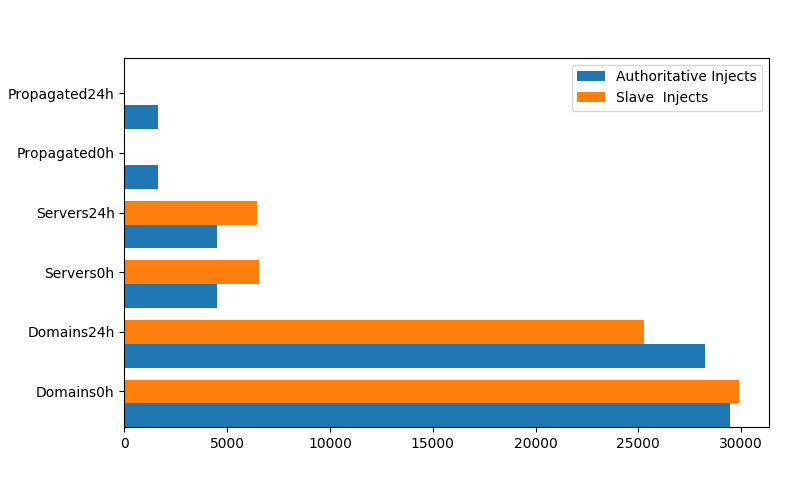
\includegraphics[width=0.8\columnwidth]{propagation}
\caption{Propagation results.}
\label{fig:propagation}
\end{figure}


We then investigate the evolution of the number of affected domains and servers over time (Table \ref{tab:propagation}).\michal{We can use Tab. \ref{tab:propagation} or Fig. \ref{fig:propagation} here} Querying affected domains directly after sending the inject reveals a similar number of domains for both primary and secondary servers. However, after 24h, the entries injected using secondary servers disappear at a much higher rate than those injected using primary servers. The entries disappear when corresponding, unaffected primary server, propagates the correct configuration to the infected secondary server. 

Furthermore, we evaluate the number of servers affected using both types of injects. Targeting primary servers results in a significantly lower number of affected servers. This is because of a higher number of secondary servers for each affected domains. The number of affected servers remains stable throughout our experiment. 

Finally, we investigate if a vulnerable server is able to infect other servers with an updated configuration. When targeting primary servers, we discovered more than 1,600 secondary servers that downloaded the incorrect zone information. We discovered a significantly lower number of secondary servers pushing changes to the primary one. This is understandable, as if configured correctly, secondary servers are not allowed to update zones. In both cases, the number of affected servers increase slightly over time. 

\subsection{Fingerprinting of vulnerable name servers}
